\documentclass{beamer}

\usepackage{amsmath}
\usepackage{mathtools}
\usepackage{amsfonts}
\usepackage{amssymb}
\usepackage{url}
\usepackage{caption}
\usepackage{subcaption}
\usepackage{svg}

\usetheme{default}

\title{Sensor Network for Smart Agriculture}
\author{Jiří Maňák}
\date{\today}

\setbeamertemplate{navigation symbols}{}
\setbeamertemplate{footline}[page number]{}
\addtobeamertemplate{footline}{
    ~~~~\small{\url{manakjiri.cz/thesis}}
}{}
\newcommand{\backupbegin}{
   \newcounter{framenumberappendix}
   \setcounter{framenumberappendix}{\value{framenumber}}
}
\newcommand{\backupend}{
   \addtocounter{framenumberappendix}{-\value{framenumber}}
   \addtocounter{framenumber}{\value{framenumberappendix}} 
}

\begin{document}

\begin{frame}
\titlepage
\end{frame}


\begin{frame}
\begin{columns}
\begin{column}{.5\textwidth}
    \begin{figure}
        \centering
        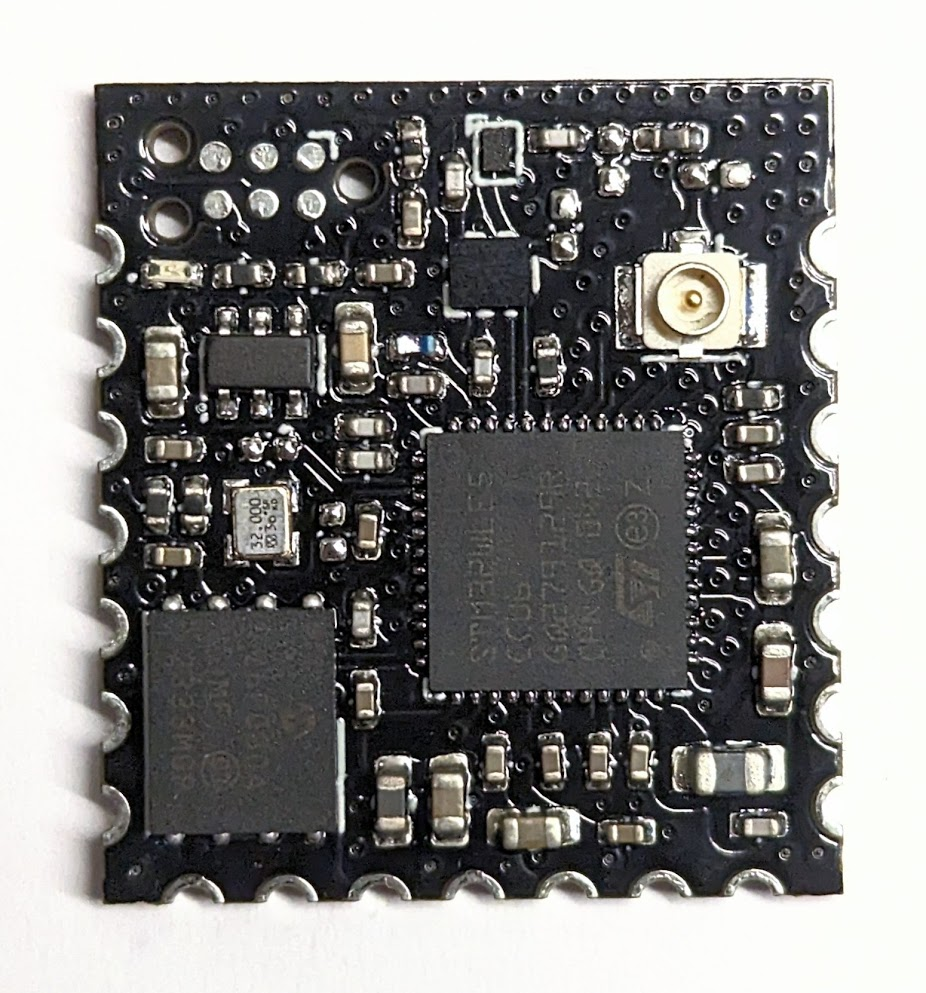
\includegraphics[width=\linewidth]{img/module-v0.1.jpg}
    \end{figure}
\end{column}
\hfil
\begin{column}{.5\textwidth}
    \begin{figure}
        \centering
        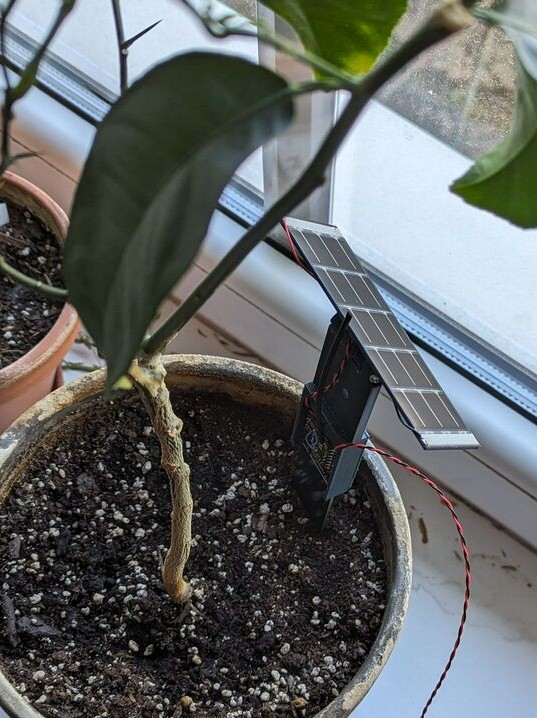
\includegraphics[width=\linewidth]{img/sensor-deploy-up.jpg}
    \end{figure}
\end{column}
\end{columns}
\end{frame}


\begin{frame}{Goals}
Custom soil moisture sensor network
\begin{itemize}
    \item Able to cover large--enough area
    \item Zero--maintenance, no external dependency
    \item Potentially extensible with more sensor types
\end{itemize}
\end{frame}

\begin{frame}{Cover large--enough area with no external dependency}
\begin{itemize}
    \item LoRa
    \item Custom protocol
\end{itemize}
\end{frame}


\begin{frame}{Zero--maintenance and extensible}
\begin{itemize}
    \item Solar power
    \item OTA updates
\end{itemize}
\end{frame}


\begin{frame}{Soil Moisture Sensor}
\begin{itemize}
    \item PCB construction
    \item 4 capacitive zones (15 cm total depth)
    \item 330 mAh lithium cell, 150 mWp solar panel
\end{itemize}
\begin{figure}
    \centering
    \includesvg[width=\linewidth]{../thesis/boards/sensor/soil-sensor-F_Cu.svg}
\end{figure}
$$\underbrace{\text{\hspace{5em}}}_{\text{Sensor electronics}}~\underbrace{\text{\hspace{19em}}}_{\text{Sensor active area}}\text{\hspace{2.5em}}$$
\end{frame}


\begin{frame}{Soil Moisture Sensor}
\centering
\begin{columns}
\begin{column}{.25\textwidth}
    \begin{flushright}
    Dielectric constant of~materials found in~soil
    \end{flushright}
\end{column}
\hfil
\begin{column}{.75\textwidth}
    \begin{figure}
        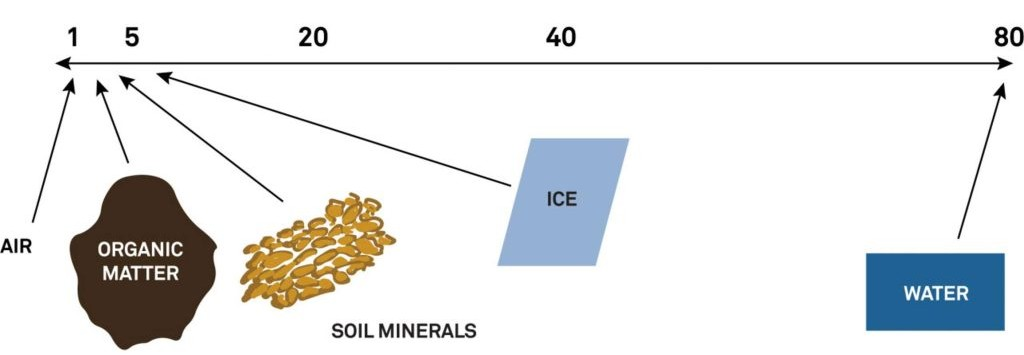
\includegraphics[width=\linewidth]{../thesis/fig/dielectric-constant.jpg}
    \end{figure}
\end{column}
\end{columns}
\begin{figure}
    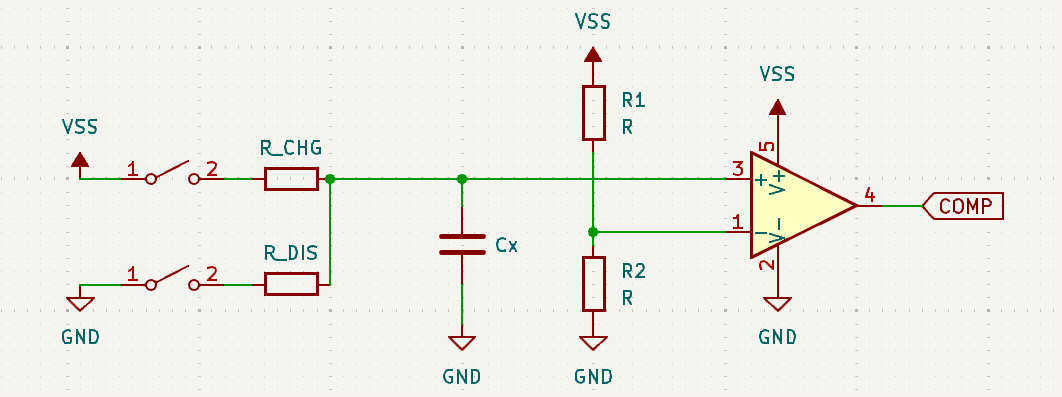
\includegraphics[width=\linewidth]{../thesis/fig/principle-cap-measure.png}
\end{figure}
\end{frame}


\begin{frame}{Soil Moisture Sensor}
\begin{columns}[T]
\begin{column}{.5\textwidth}
    \begin{figure}
        \centering
        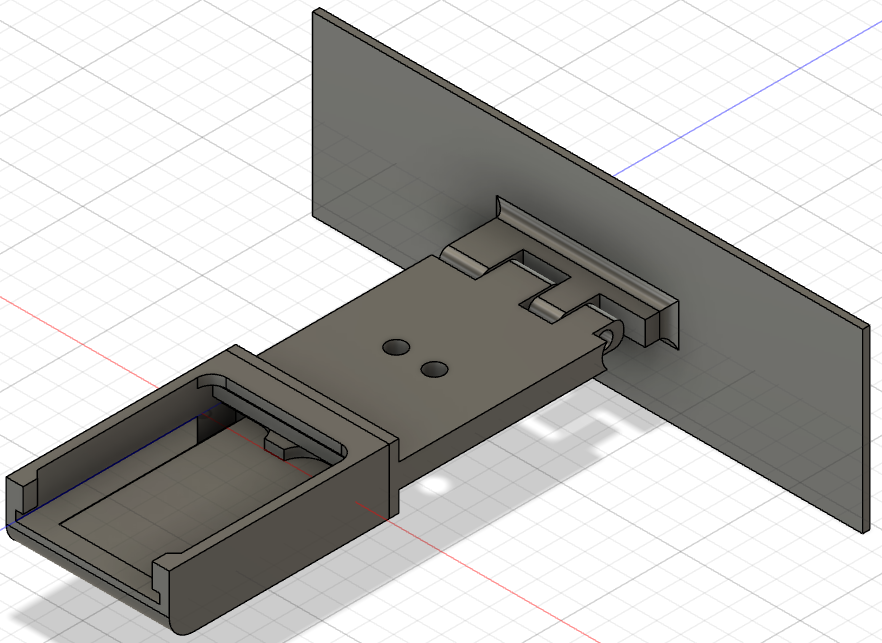
\includegraphics[width=\linewidth]{../thesis/img/sensor-case.png}
    \end{figure}
\end{column}
\hfil
\begin{column}{.5\textwidth}
    \begin{figure}
        \centering
        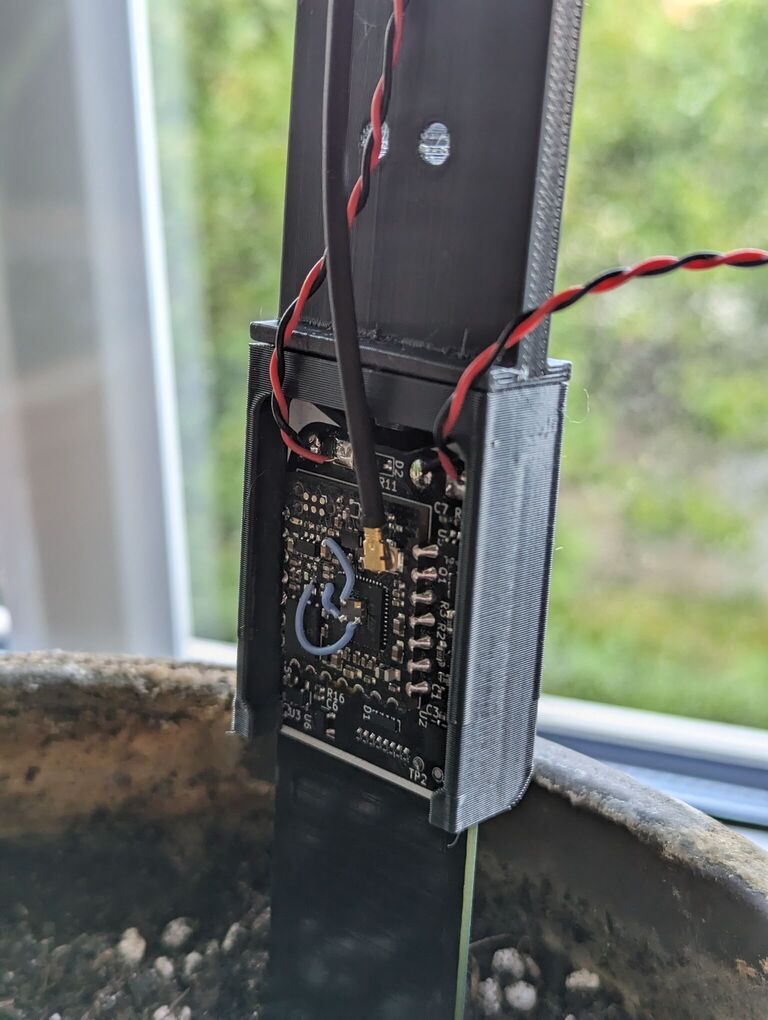
\includegraphics[width=\linewidth]{../thesis/img/sensor-deploy-close.jpg}
    \end{figure}
\end{column}
\end{columns}
\end{frame}


\begin{frame}{LoRa Module}
\begin{figure}
    \centering
    \small
    \includesvg[width=.8\linewidth]{img/module-v0.1.drawio.svg}
\end{figure}
\begin{columns}[T]
\begin{column}{.5\textwidth}
    \begin{itemize}
        \item \textbf{STM32WLE5CC}
        \item 868 MHz, 15 dBm
        \item \textbf{20.32}$\mathbf{\times}$\textbf{22.48 mm}
    \end{itemize}
\end{column}
\hfill
\begin{column}{.5\textwidth}
    \begin{itemize}
        \item 1 MB FLASH
        \item 2.3--3.5 V
        \item 16 IO pins
    \end{itemize}
\end{column}
\end{columns}
\end{frame}


\begin{frame}{LoRa Module Range Test}
\begin{columns}[T]
\begin{column}{.3\textwidth}
    \centering
    \begin{figure}
        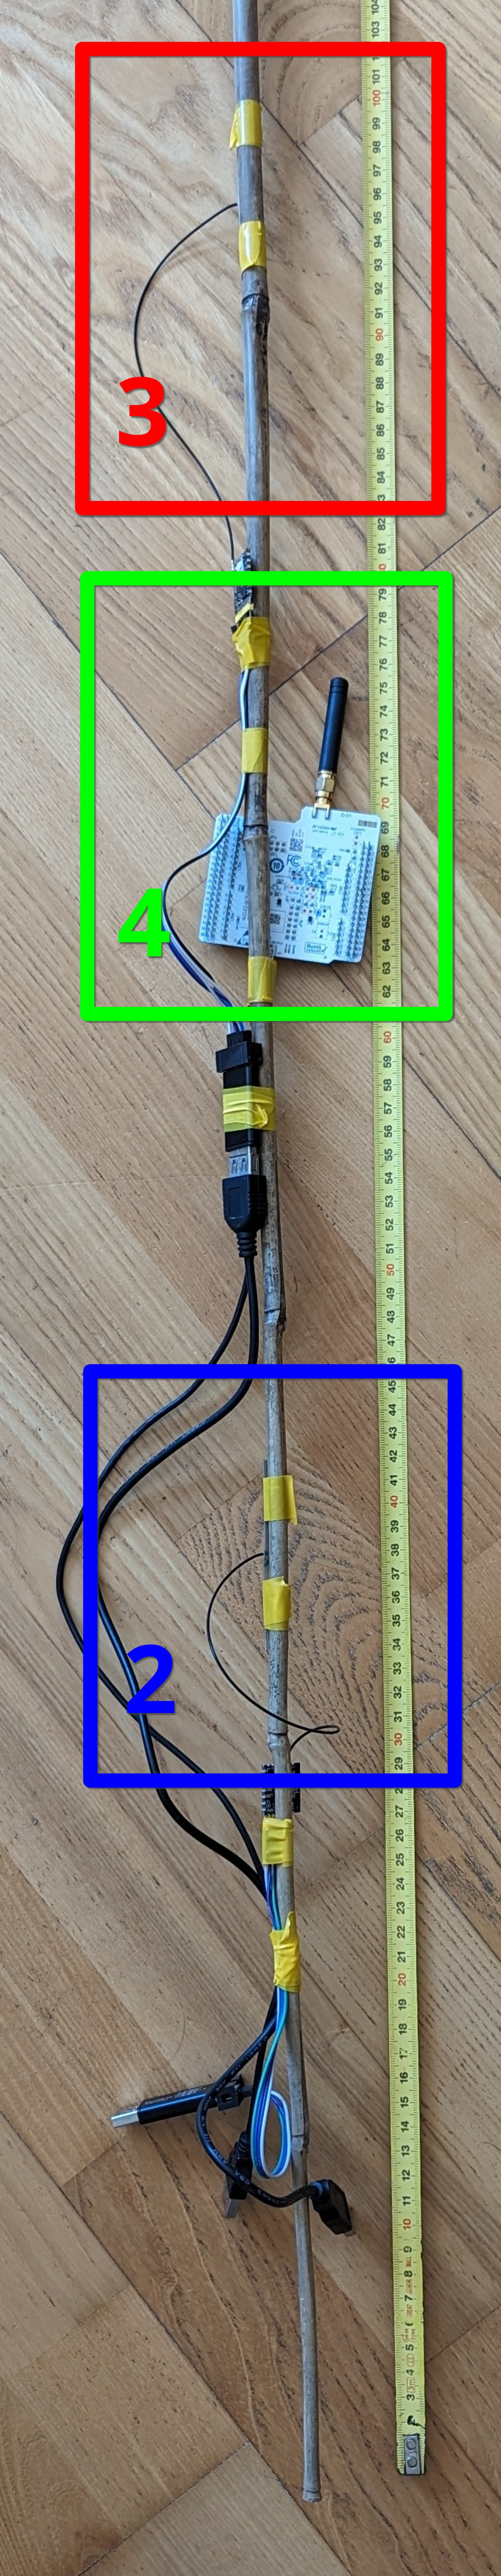
\includegraphics[height=7.5cm]{img/lora-pole.jpg}
    \end{figure}
\end{column}
\hfil
\begin{column}{.3\textwidth}
    \centering
    \begin{figure}
        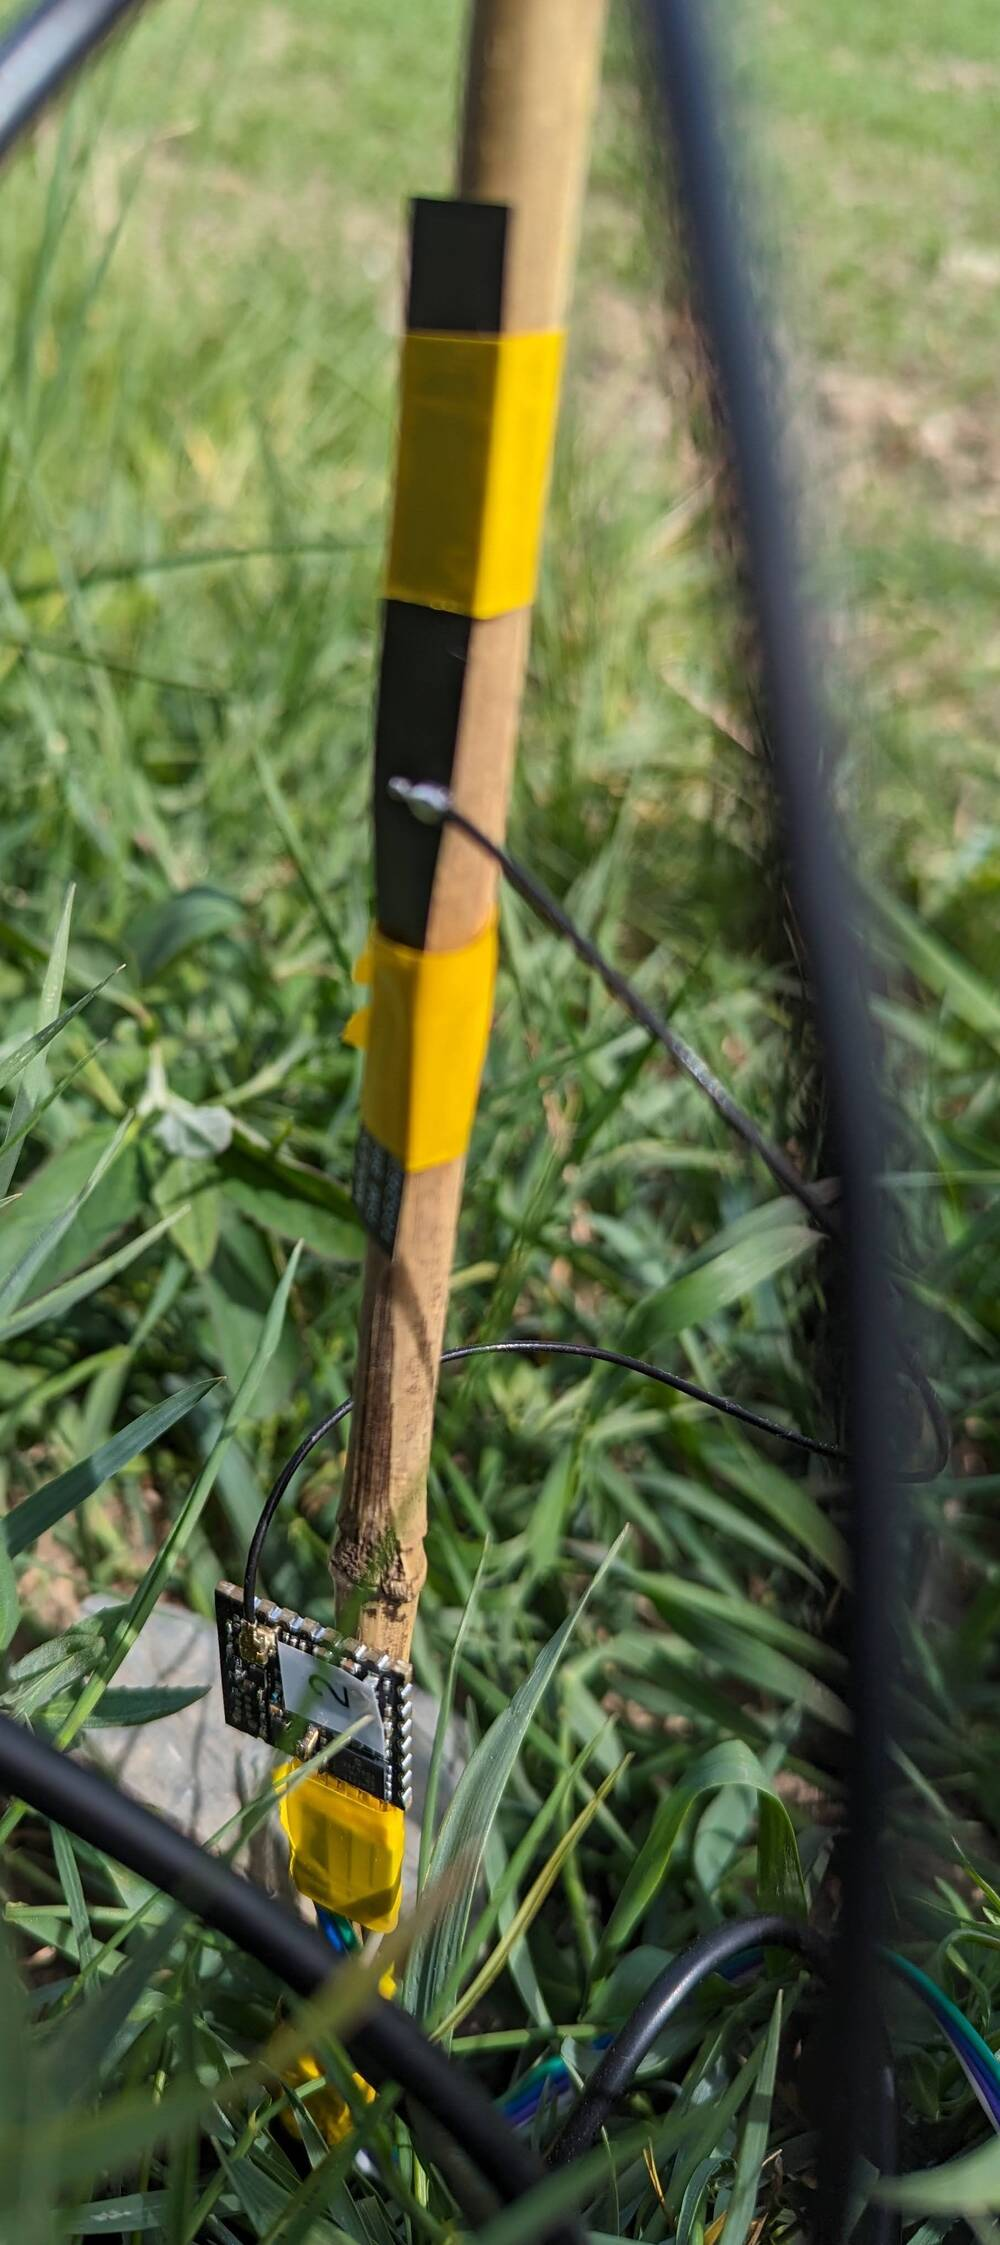
\includegraphics[height=7cm]{../thesis/img/range-pole-bottom.jpg}
    \end{figure}
    \vspace{-1em}
    Node 2
\end{column}
\hfil
\begin{column}{.3\textwidth}
    \centering
    \begin{figure}
        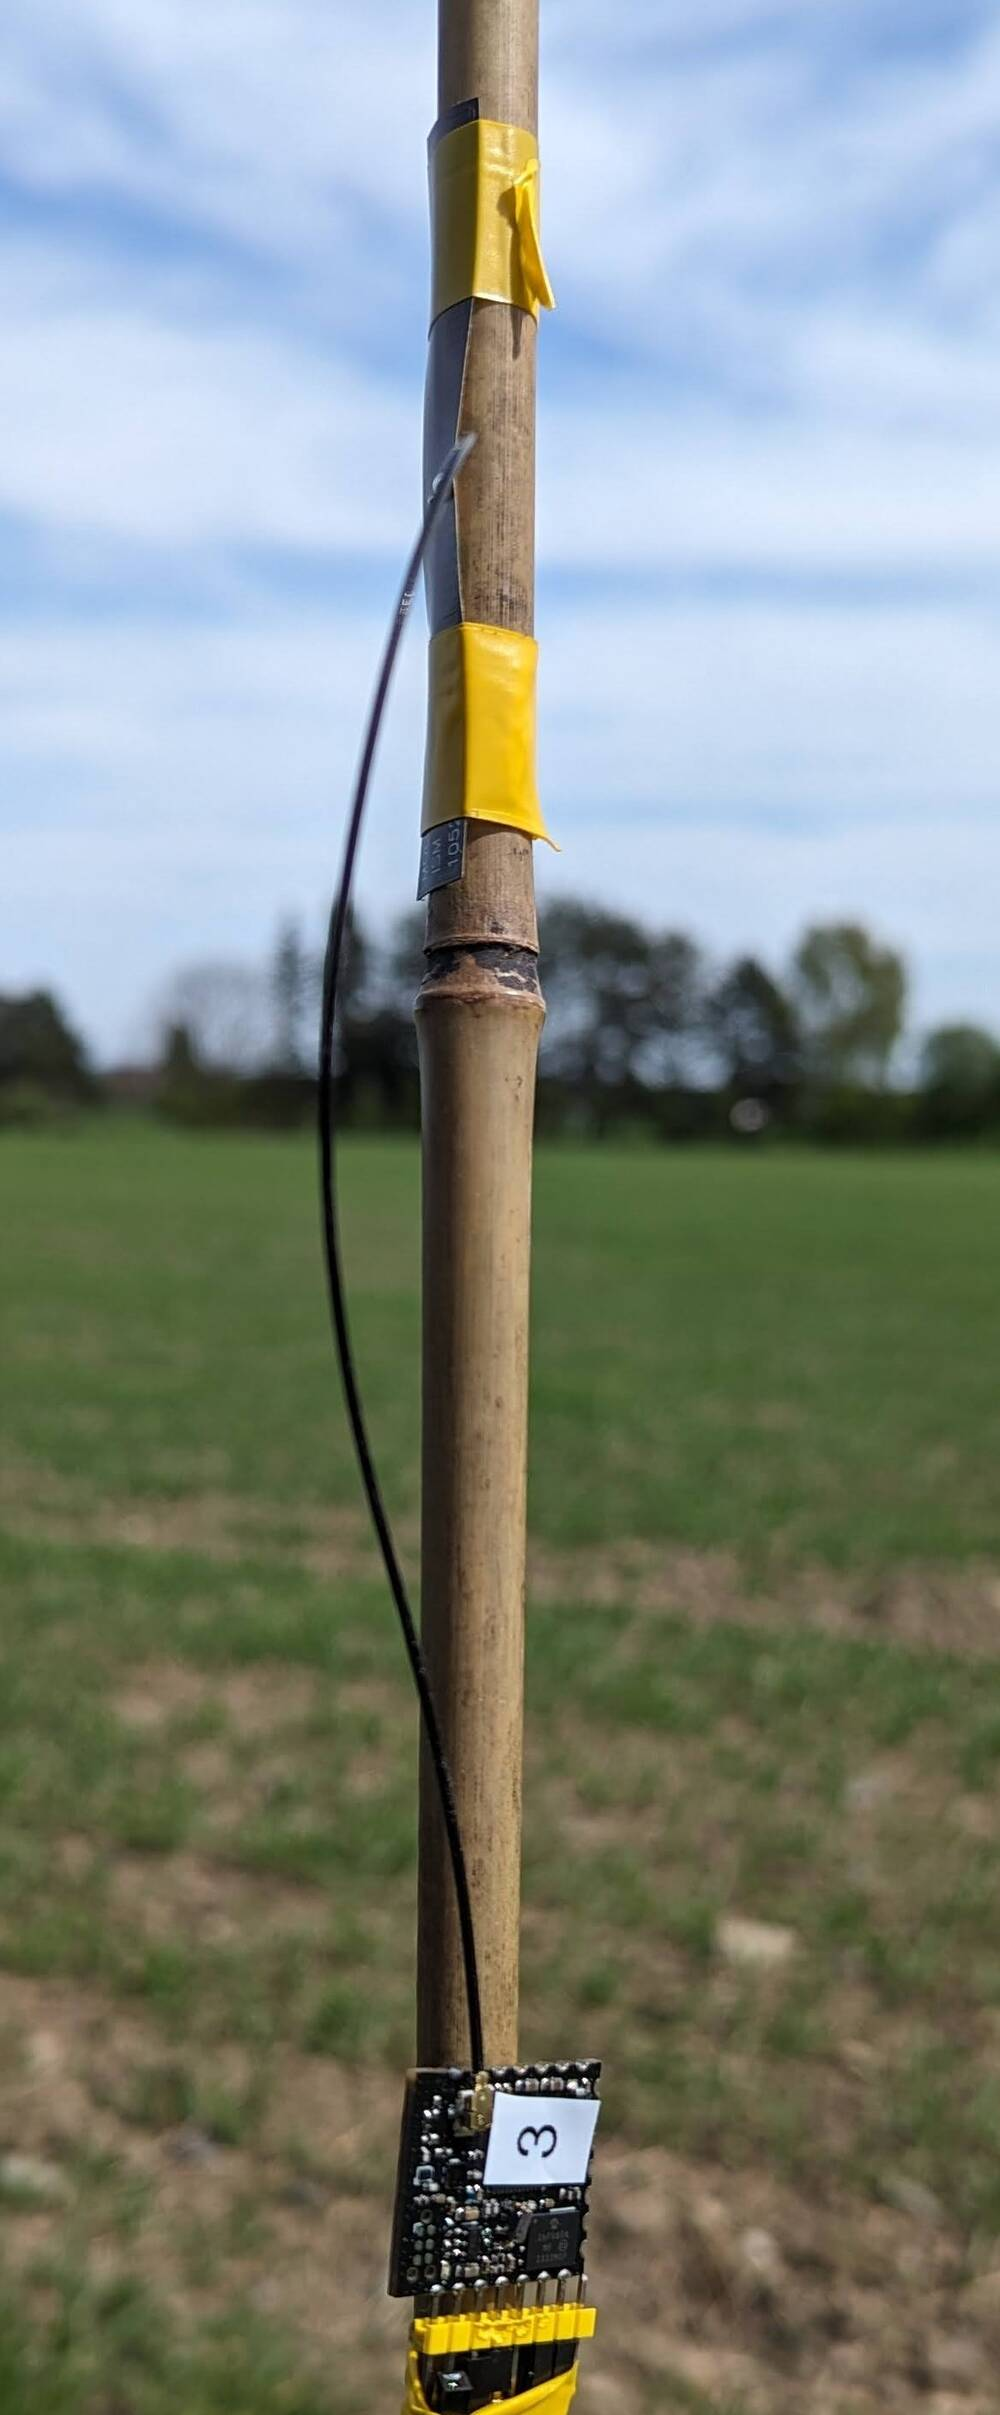
\includegraphics[height=7cm]{../thesis/img/range-pole-top.jpg}
    \end{figure}
    \vspace{-1em}
    Node 3
\end{column}
\end{columns}
\end{frame}


\begin{frame}{LoRa Module Range Test - SF11}
\begin{figure}
    \includesvg[width=\linewidth]{../thesis/data/range/out/success-sf11.svg}
\end{figure}
\begin{figure}
    \includesvg[width=\linewidth]{../thesis/data/range/out/relief-sf11.svg}
\end{figure}
\Tiny{\textbf{Node 2 - 20 cm, Node 3 - 80 cm, Node 4 (Nucleo) - 50 cm}, 1.125 s round-trip, 300 bps, Page 41, Section 4.4.4}
\end{frame}

\begin{frame}{LoRa Module Range Test - SF5}
\begin{figure}
    \includesvg[width=\linewidth]{../thesis/data/range/out/success-sf5.svg}
\end{figure}
\begin{figure}
    \includesvg[width=\linewidth]{../thesis/data/range/out/relief-sf5.svg}
\end{figure}
\Tiny{\textbf{Node 2 - 20 cm, Node 3 - 80 cm, Node 4 (Nucleo) - 50 cm}, 0.125 s round-trip, 3 kbps, Page 41, Section 4.4.4}
\end{frame}


\begin{frame}{Soil Moisture Sensor Validation}
\begin{figure}
    \includesvg[width=\linewidth]{../thesis/data/deployment/out/moisture-cal.svg}
\end{figure}
\end{frame}


\begin{frame}{Live Demo}
\begin{figure}
    \centering
    
\includegraphics[width=.5\linewidth]{img/qr.png}
\end{figure}
\begin{center}
    (or visit the link)
\end{center}
\end{frame}


\begin{frame}{Conclusion}
This thesis brought
\begin{itemize}
    \item \textbf{STM32 LoRa Module - a platform for connected sensors}
    \item \textbf{Soil moisture sensor - an application of the module}
    \item Backend service which processes the sensor data
    \item \url{module-runtime} Rust package - HAL, OTA, async
\end{itemize}
\vspace{1em}
All publicly available at \url{https://github.com/manakjiri}
\end{frame}

\appendix
\backupbegin


\begin{frame}{LoRa Module}
\begin{figure}
    \centering
    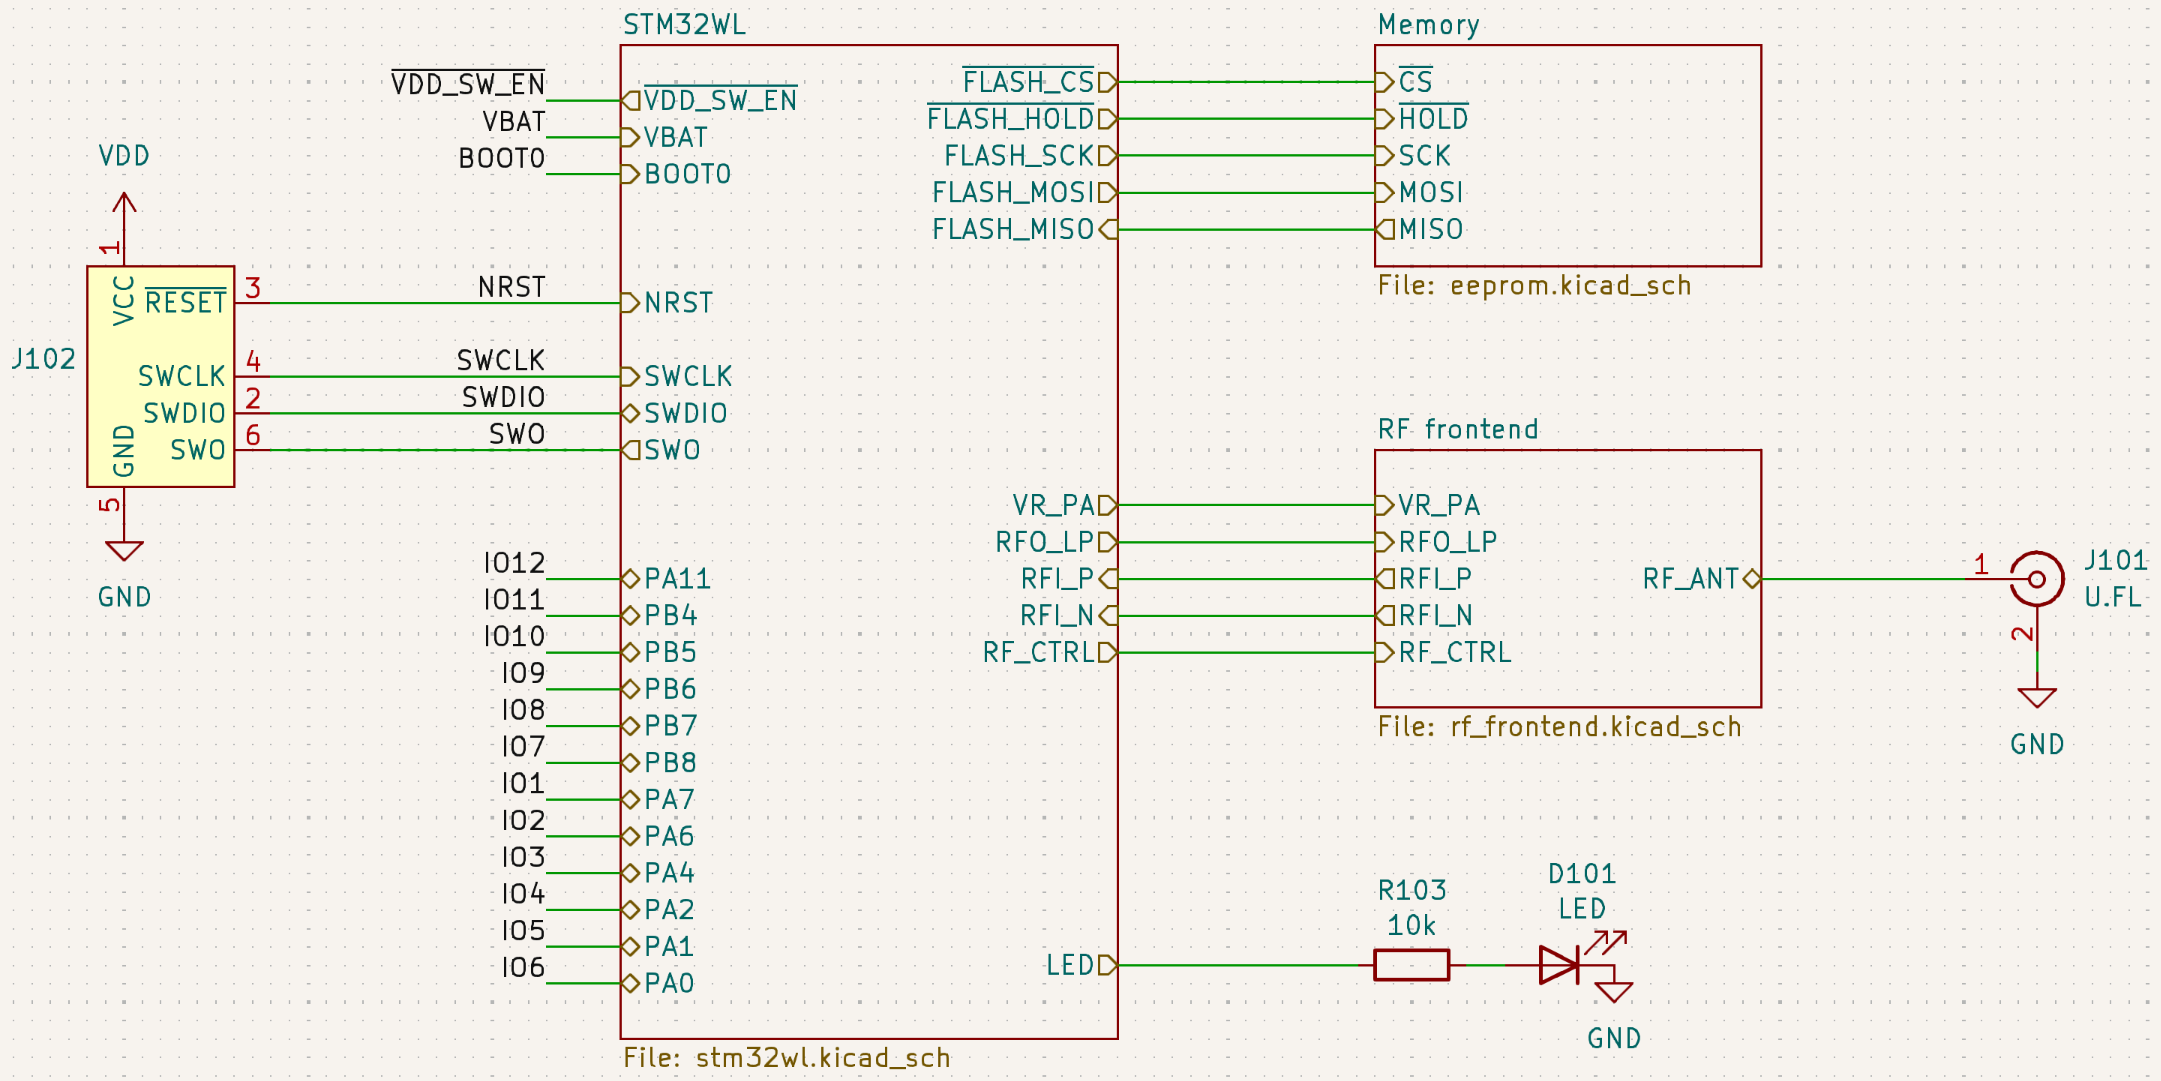
\includegraphics[width=\linewidth]{img/module-schema.png}
\end{figure}
\end{frame}


\begin{frame}{LoRa Module}
\begin{columns}[T]
\begin{column}{.3\textwidth}
    \centering
    \begin{figure}
        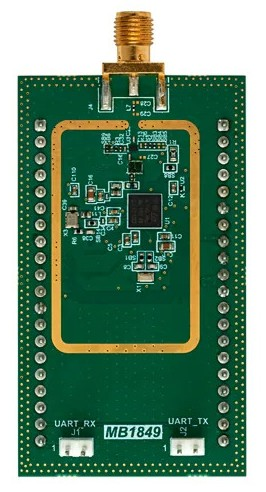
\includegraphics[width=.9\linewidth]{img/STDES-WL5U4ILH.jpg}
    \end{figure}
    STDES-WL5U4ILH
\end{column}
\hfil
\begin{column}{.3\textwidth}
    \centering
    \begin{figure}
        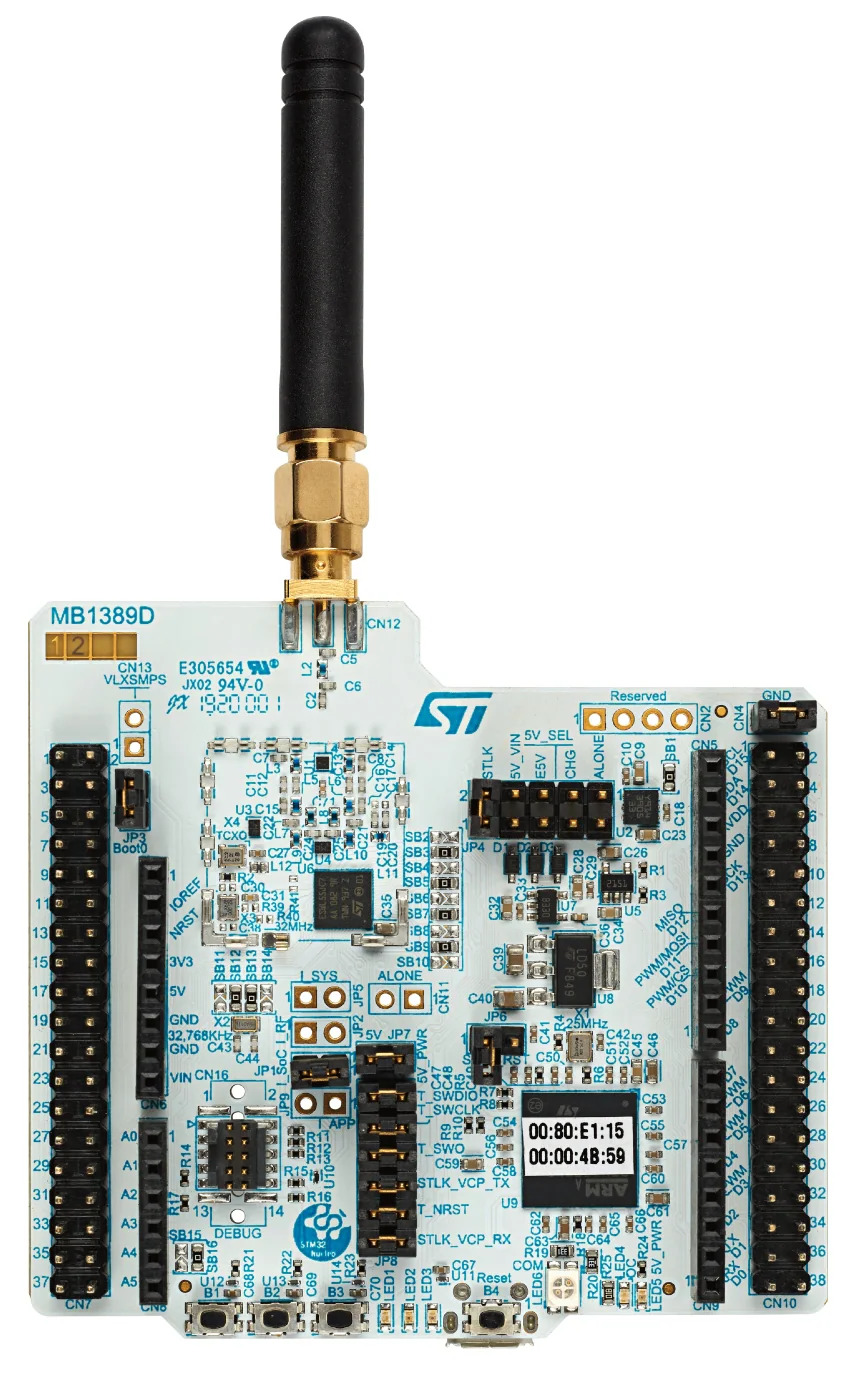
\includegraphics[width=\linewidth]{img/nucleo-wl55jc.jpg}
    \end{figure}
    Nucleo-WL55JC
\end{column}
\end{columns}
\end{frame}


\begin{frame}{Existing solution?}
\begin{columns}
\begin{column}{.4\textwidth}
    \centering
    \begin{figure}
        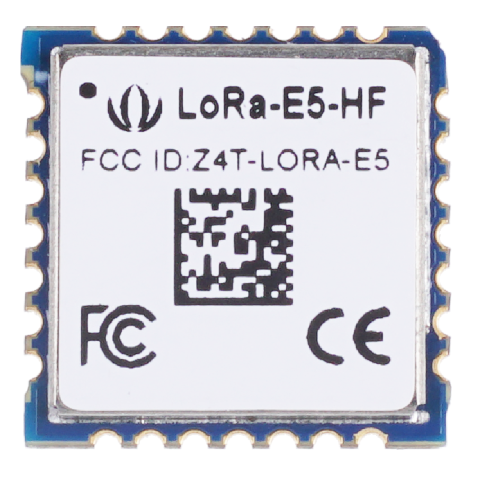
\includegraphics[width=\linewidth]{img/wio-e5.png}
    \end{figure}
    Seeed Studio Wio-E5
\end{column}
\hfil
\begin{column}{.1\textwidth}
    \centering
    \Large
    \vspace{-2em}
    $$>$$
    ?
    $$<$$
\end{column}
\hfil
\begin{column}{.4\textwidth}
    \centering
    \begin{figure}
        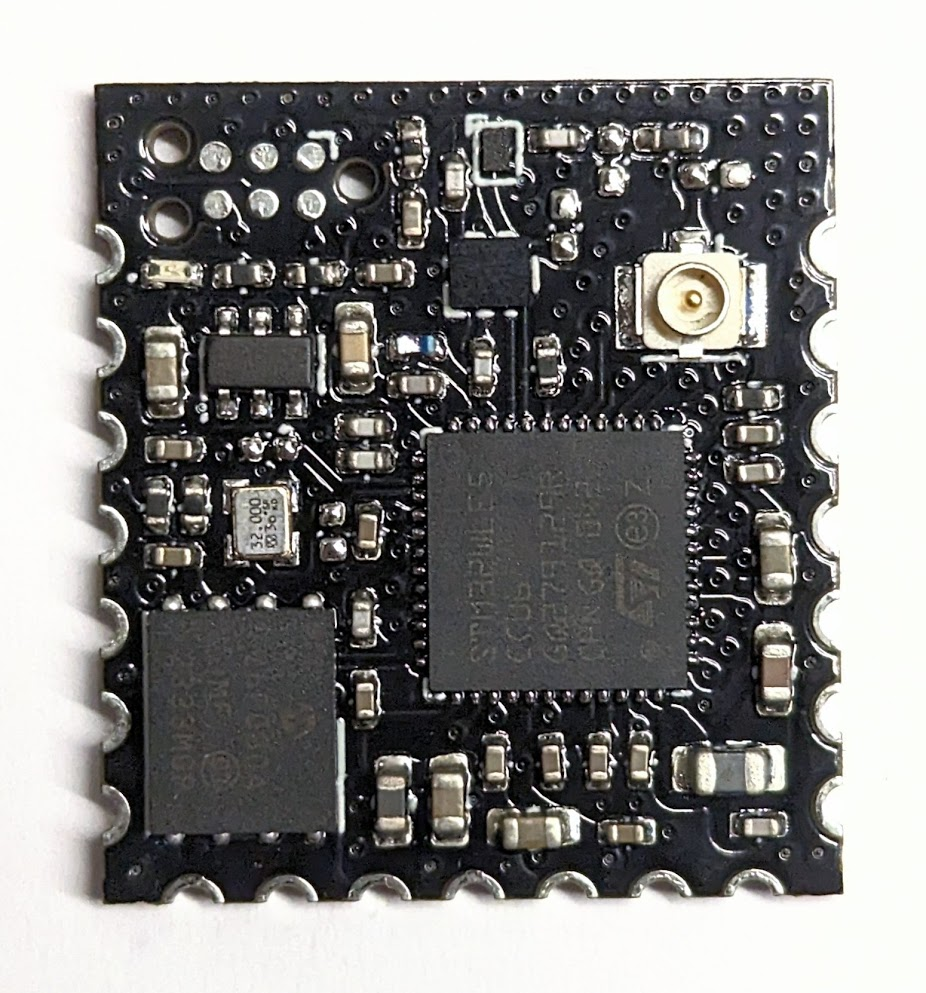
\includegraphics[width=\linewidth]{img/module-v0.1.jpg}
    \end{figure}
    My LoRa Module
\end{column}
\end{columns}
\end{frame}


\begin{frame}{Solar Power}
\begin{figure}
    \includesvg[width=\linewidth]{../thesis/data/deployment/out/power.svg}
\end{figure}
\end{frame}

\begin{frame}{Firmware}
\begin{figure}
    \centering
    \includesvg[width=\linewidth]{img/firmware.drawio.svg}
\end{figure}
\end{frame}


\begin{frame}{Over The Air Update}
\begin{figure}
    \centering
    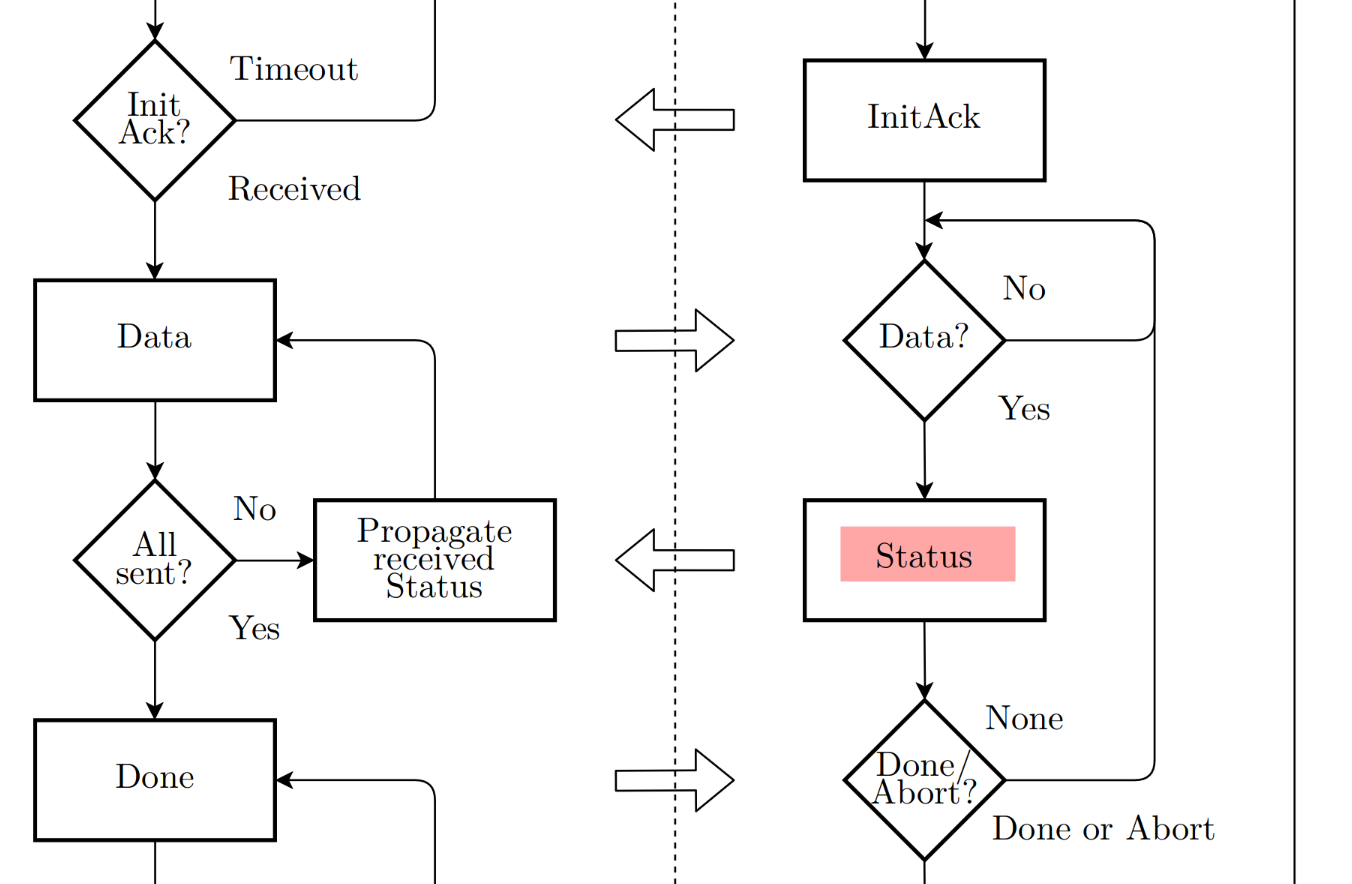
\includegraphics[width=\linewidth]{img/ota.png}
\end{figure}
\begin{flushright}
    Page 36, Figure 4.9
\end{flushright}
\end{frame}


\begin{frame}{LoRa Module}
\begin{itemize}
    \item 2.8--3.3 V nominal voltage range,
    \item low power design - support for switchable power rails,
    \item target the EU868,
    \item wide temperature range
    \item minimize the amount of specialized hardware,
    \item support for OTA updates,
    \item integrated RF,
    \item host communication interface,
    \item minimal footprint,
    \item low cost.
\end{itemize}
\begin{flushright}
    Page 15, Section 3.2.3
\end{flushright}
\end{frame}

\backupend

\end{document}
